\documentclass{article}
\usepackage{tikz}
\usetikzlibrary{arrows.meta,positioning,calc,shapes.geometric}
\pagestyle{empty}
\begin{document}
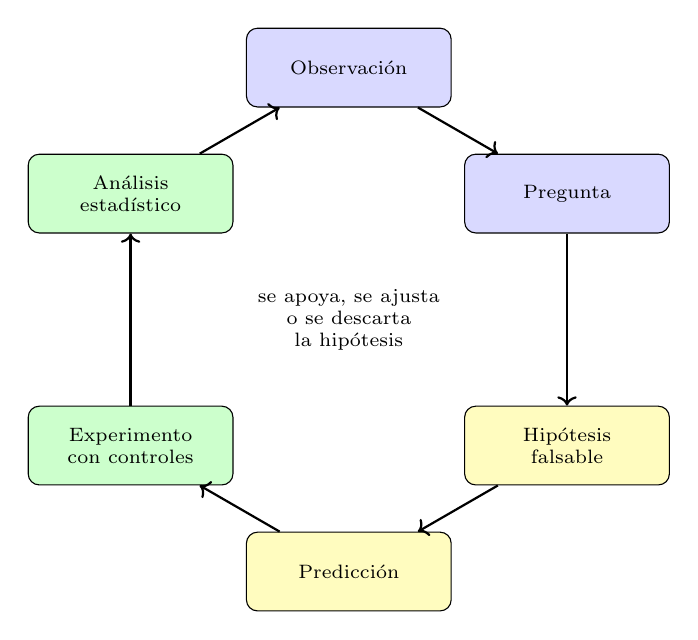
\begin{tikzpicture}
\tikzset{every node/.append style={align=center}}

\foreach \a/\t/\c in {90/Observación/blue!15, 30/Pregunta/blue!15, -30/Hipótesis\\ falsable/yellow!25, -90/Predicción/yellow!25, -150/Experimento\\ con controles/green!20, 150/Análisis\\ estadístico/green!20} {
  \node[draw, rounded corners, fill=\c, minimum width=2.6cm, minimum height=1.0cm, align=center, font=\scriptsize] (n\a) at (\a:3.2) {\t};}
\draw[->, thick] (n90) -- (n30); \draw[->, thick] (n30) -- (n-30); \draw[->, thick] (n-30) -- (n-90); \draw[->, thick] (n-90) -- (n-150); \draw[->, thick] (n-150) -- (n150); \draw[->, thick] (n150) -- (n90);
\node[font=\scriptsize, align=center] at (0,0) {se apoya, se ajusta\\ o se descarta\\ la hipótesis};

\end{tikzpicture}
\end{document}
